\documentclass[onecolumn]{article}
\usepackage{graphicx}
\usepackage[utf8]{inputenc} % UTF8 input encoding
\usepackage{microtype} % bedre orddeling & andet typografisk halløj
\usepackage{amsmath, amssymb, mathtools, bm, nicefrac, mathrsfs} % matematik-pakker
\raggedbottom
\newcommand{\sub}[1]{_{\mathrm{#1}}}

\begin{document}
\title{Exam Project: Exercise 15 - Generalizing an ODE solver to the Complex Plane}
\date{}
\author{Mikkel Elkjaer Pedersen}
\maketitle

This short report presents my reflections on the exam exercise 15: \textit{Generalize the ODE solver of your choice to solve ODE with 
complex-valued functions of complex variable along a straight line between the given start- and end-point}.
As this exam project is an extension of the ODE-exercise in the course I have reused large parts of the code from my ODE-solver.
Thus, this ODE-solver also utilizes a Runge-Kutta23 stepper as the advancing mechanism, also called the Bogacki-Shampine method. \\

My first consideration in this project was how to modify the working ODE-solver for real functions to complex functions, that is,
what is the most natural way to incorporate the imaginary part into the already established part. A first thought was to exploit that the
solver already works for any number of variables. In this sense one might \textit{pair up} variables where each pair would represent the
real and complex parts of a single complex variable, respectively. Even though this seems like a natural way of solving the problem I could 
not convince myself that this would work in general as complex functions of complex variables in general "mixes" the two parts. 
As an example, squaring a complex number with a non-zero imaginary part intricately affects the real part, which might even be negative, 
and therefore i quickly abandoned this approach. The much safer approach, although more cumbersome in typing, is to just cast every variable 
as complex from the very start. To do this i chose to utilize the GSL-library representation. The price of the build-in complex
arithmetic functions is of course the famously long function names of GSL-routines. Looking back at the resulting code after implementing 
these modifications I believe it would have been just as easy to use my own small library for dealing with complex variables from the 
exercise called "komplex".\\

With regards to the mathematics in the modifications not many comments are necessary as the Runge-Kutta methods nowhere assume real variables. 
Thus adhering to the arithmetics of complex numbers should leave a proper algorithm. 
Most notable is the caution one must show when considering the step, $\mathrm{h}$, as the meaning of a step and the step size coincide in 
one dimension, that is for real variables, but not for two dimensions. Thus the step sought by the driver for a complex function of a 
complex variable is a complex number, while the step size naturally remains a real number.\\

As in part B of the ODE-exercise in the course I have retained the property that the solver saves the steps validated by the driver and the 
corresponding function values. For this part I have one reflection. This concerns the fact that the user must supply an upper limit to how many 
steps that is considered feasible for the driver to take. If the upper limit of the integration of the ODE is not reached within this limit 
an indication is send to the output along with the steps and function values that were reached before the count limit. Of course this allows 
the user to restart the solver at the reached point untill completion but if this is repeatedly necessary this a hardly flexible driver. 
Also, establishing an upper limit has the clear disadvantage that the user must somehow be able to ballpark the necessary number of steps 
before the routine is run. In general, the user should then also overestimate the required number of steps just to be safe. For complecated
problem this might lead to serious overestimates and in consequence unnecessarily huge collector matrices to be handled by the driver which
could slow the routine quite significantly. For such complicated problems the user relies heavily on restarting the driver and storing the 
results in between restarts. The stored path might also be used to reveal treacherous or seamless sub-regions for which a more or less demanding 
accuracy should be supplied to the driver before a total restart. \\

To demonstrate that my routine works I have solved three very simple problems. The first is in fact a purely real problem meant as an explicit 
display that real problems may of course also be handled by this complex driver. Thus, as seen in figure \ref{fig:real}, the real exponential 
function is determined by its ODE-representation $\mathrm{dy/dt} = y$ with initial condition $y(0)=1$.
Secondly, the ODE for the complex exponential function along the imaginary axis is used to produce the purple and blue graphs in figure 
\ref{fig:complex}. Do note that the imaginary part is strictly 0 all throughout as it should be.
Lastly, the ODE for the complex exponential function along the real axis is integrated up to $2\pi$ to show one revolution 
of the sine and cosine functions which are of course the imaginary and real parts of the complex exponential, respectively. The result is 
included in figure \ref{fig:complex}.

As stated in the exercise description the integration of the ODE should be along a straight line in the complex plain. To ensure this I have 
implemented an enforcer of this restriction into the driver routine. That is, when the user has supplied a start and end point of the straight 
line for which the driver should solve the ODE the user is also required to supply an initial guess of the first step the driver should take. 
Regardless of whether this guess is in fact in the correct direction the driver now extracts the approximate size of the intended first step 
in both the real and imaginary direction, separately. It then calculates an initial guess in the correct direction which is on the scale of the 
user guess for each direction, separately. Thus all directions in the complex plain should be solvable for the driver if the user provides 
the correct ODE even though a very misleading initial step guess is provided. 


\begin{figure}
% GNUPLOT: LaTeX picture with Postscript
\begingroup
  \makeatletter
  \providecommand\color[2][]{%
    \GenericError{(gnuplot) \space\space\space\@spaces}{%
      Package color not loaded in conjunction with
      terminal option `colourtext'%
    }{See the gnuplot documentation for explanation.%
    }{Either use 'blacktext' in gnuplot or load the package
      color.sty in LaTeX.}%
    \renewcommand\color[2][]{}%
  }%
  \providecommand\includegraphics[2][]{%
    \GenericError{(gnuplot) \space\space\space\@spaces}{%
      Package graphicx or graphics not loaded%
    }{See the gnuplot documentation for explanation.%
    }{The gnuplot epslatex terminal needs graphicx.sty or graphics.sty.}%
    \renewcommand\includegraphics[2][]{}%
  }%
  \providecommand\rotatebox[2]{#2}%
  \@ifundefined{ifGPcolor}{%
    \newif\ifGPcolor
    \GPcolortrue
  }{}%
  \@ifundefined{ifGPblacktext}{%
    \newif\ifGPblacktext
    \GPblacktexttrue
  }{}%
  % define a \g@addto@macro without @ in the name:
  \let\gplgaddtomacro\g@addto@macro
  % define empty templates for all commands taking text:
  \gdef\gplbacktext{}%
  \gdef\gplfronttext{}%
  \makeatother
  \ifGPblacktext
    % no textcolor at all
    \def\colorrgb#1{}%
    \def\colorgray#1{}%
  \else
    % gray or color?
    \ifGPcolor
      \def\colorrgb#1{\color[rgb]{#1}}%
      \def\colorgray#1{\color[gray]{#1}}%
      \expandafter\def\csname LTw\endcsname{\color{white}}%
      \expandafter\def\csname LTb\endcsname{\color{black}}%
      \expandafter\def\csname LTa\endcsname{\color{black}}%
      \expandafter\def\csname LT0\endcsname{\color[rgb]{1,0,0}}%
      \expandafter\def\csname LT1\endcsname{\color[rgb]{0,1,0}}%
      \expandafter\def\csname LT2\endcsname{\color[rgb]{0,0,1}}%
      \expandafter\def\csname LT3\endcsname{\color[rgb]{1,0,1}}%
      \expandafter\def\csname LT4\endcsname{\color[rgb]{0,1,1}}%
      \expandafter\def\csname LT5\endcsname{\color[rgb]{1,1,0}}%
      \expandafter\def\csname LT6\endcsname{\color[rgb]{0,0,0}}%
      \expandafter\def\csname LT7\endcsname{\color[rgb]{1,0.3,0}}%
      \expandafter\def\csname LT8\endcsname{\color[rgb]{0.5,0.5,0.5}}%
    \else
      % gray
      \def\colorrgb#1{\color{black}}%
      \def\colorgray#1{\color[gray]{#1}}%
      \expandafter\def\csname LTw\endcsname{\color{white}}%
      \expandafter\def\csname LTb\endcsname{\color{black}}%
      \expandafter\def\csname LTa\endcsname{\color{black}}%
      \expandafter\def\csname LT0\endcsname{\color{black}}%
      \expandafter\def\csname LT1\endcsname{\color{black}}%
      \expandafter\def\csname LT2\endcsname{\color{black}}%
      \expandafter\def\csname LT3\endcsname{\color{black}}%
      \expandafter\def\csname LT4\endcsname{\color{black}}%
      \expandafter\def\csname LT5\endcsname{\color{black}}%
      \expandafter\def\csname LT6\endcsname{\color{black}}%
      \expandafter\def\csname LT7\endcsname{\color{black}}%
      \expandafter\def\csname LT8\endcsname{\color{black}}%
    \fi
  \fi
    \setlength{\unitlength}{0.0500bp}%
    \ifx\gptboxheight\undefined%
      \newlength{\gptboxheight}%
      \newlength{\gptboxwidth}%
      \newsavebox{\gptboxtext}%
    \fi%
    \setlength{\fboxrule}{0.5pt}%
    \setlength{\fboxsep}{1pt}%
\begin{picture}(7200.00,4320.00)%
    \gplgaddtomacro\gplbacktext{%
      \csname LTb\endcsname%%
      \put(543,595){\makebox(0,0)[r]{\strut{}$0$}}%
      \csname LTb\endcsname%%
      \put(543,917){\makebox(0,0)[r]{\strut{}$2$}}%
      \csname LTb\endcsname%%
      \put(543,1238){\makebox(0,0)[r]{\strut{}$4$}}%
      \csname LTb\endcsname%%
      \put(543,1560){\makebox(0,0)[r]{\strut{}$6$}}%
      \csname LTb\endcsname%%
      \put(543,1882){\makebox(0,0)[r]{\strut{}$8$}}%
      \csname LTb\endcsname%%
      \put(543,2203){\makebox(0,0)[r]{\strut{}$10$}}%
      \csname LTb\endcsname%%
      \put(543,2525){\makebox(0,0)[r]{\strut{}$12$}}%
      \csname LTb\endcsname%%
      \put(543,2846){\makebox(0,0)[r]{\strut{}$14$}}%
      \csname LTb\endcsname%%
      \put(543,3168){\makebox(0,0)[r]{\strut{}$16$}}%
      \csname LTb\endcsname%%
      \put(543,3490){\makebox(0,0)[r]{\strut{}$18$}}%
      \csname LTb\endcsname%%
      \put(543,3811){\makebox(0,0)[r]{\strut{}$20$}}%
      \csname LTb\endcsname%%
      \put(543,4133){\makebox(0,0)[r]{\strut{}$22$}}%
      \csname LTb\endcsname%%
      \put(645,409){\makebox(0,0){\strut{}$0$}}%
      \csname LTb\endcsname%%
      \put(1686,409){\makebox(0,0){\strut{}$0.5$}}%
      \csname LTb\endcsname%%
      \put(2728,409){\makebox(0,0){\strut{}$1$}}%
      \csname LTb\endcsname%%
      \put(3769,409){\makebox(0,0){\strut{}$1.5$}}%
      \csname LTb\endcsname%%
      \put(4810,409){\makebox(0,0){\strut{}$2$}}%
      \csname LTb\endcsname%%
      \put(5852,409){\makebox(0,0){\strut{}$2.5$}}%
      \csname LTb\endcsname%%
      \put(6893,409){\makebox(0,0){\strut{}$3$}}%
    }%
    \gplgaddtomacro\gplfronttext{%
      \csname LTb\endcsname%%
      \put(153,2364){\rotatebox{-270}{\makebox(0,0){\strut{}y}}}%
      \csname LTb\endcsname%%
      \put(3769,130){\makebox(0,0){\strut{}x}}%
      \csname LTb\endcsname%%
      \put(2583,3966){\makebox(0,0)[r]{\strut{}Real exp from ODE}}%
      \csname LTb\endcsname%%
      \put(2583,3780){\makebox(0,0)[r]{\strut{}Exp(x) from math.h}}%
    }%
    \gplbacktext
    \put(0,0){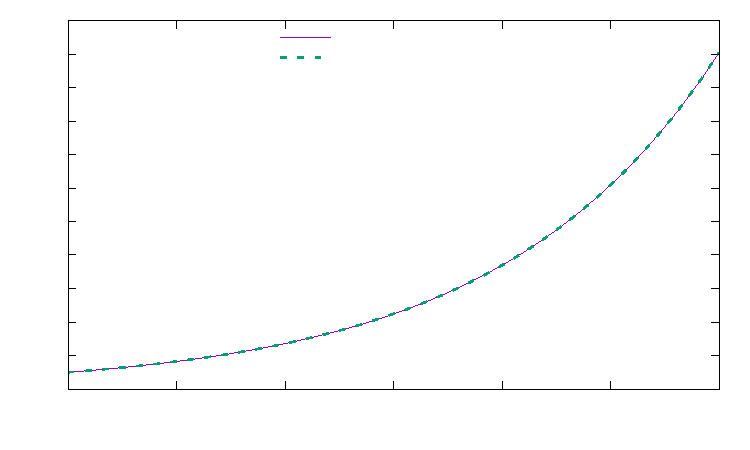
\includegraphics{plot_real}}%
    \gplfronttext
  \end{picture}%
\endgroup

        \caption{A plot of the ODE representation of the real exponential function and the one from the standard C library math.h in the range
                $[0,3]$.}
\label{fig:real}
\end{figure}

\begin{figure}
% GNUPLOT: LaTeX picture with Postscript
\begingroup
  \makeatletter
  \providecommand\color[2][]{%
    \GenericError{(gnuplot) \space\space\space\@spaces}{%
      Package color not loaded in conjunction with
      terminal option `colourtext'%
    }{See the gnuplot documentation for explanation.%
    }{Either use 'blacktext' in gnuplot or load the package
      color.sty in LaTeX.}%
    \renewcommand\color[2][]{}%
  }%
  \providecommand\includegraphics[2][]{%
    \GenericError{(gnuplot) \space\space\space\@spaces}{%
      Package graphicx or graphics not loaded%
    }{See the gnuplot documentation for explanation.%
    }{The gnuplot epslatex terminal needs graphicx.sty or graphics.sty.}%
    \renewcommand\includegraphics[2][]{}%
  }%
  \providecommand\rotatebox[2]{#2}%
  \@ifundefined{ifGPcolor}{%
    \newif\ifGPcolor
    \GPcolortrue
  }{}%
  \@ifundefined{ifGPblacktext}{%
    \newif\ifGPblacktext
    \GPblacktexttrue
  }{}%
  % define a \g@addto@macro without @ in the name:
  \let\gplgaddtomacro\g@addto@macro
  % define empty templates for all commands taking text:
  \gdef\gplbacktext{}%
  \gdef\gplfronttext{}%
  \makeatother
  \ifGPblacktext
    % no textcolor at all
    \def\colorrgb#1{}%
    \def\colorgray#1{}%
  \else
    % gray or color?
    \ifGPcolor
      \def\colorrgb#1{\color[rgb]{#1}}%
      \def\colorgray#1{\color[gray]{#1}}%
      \expandafter\def\csname LTw\endcsname{\color{white}}%
      \expandafter\def\csname LTb\endcsname{\color{black}}%
      \expandafter\def\csname LTa\endcsname{\color{black}}%
      \expandafter\def\csname LT0\endcsname{\color[rgb]{1,0,0}}%
      \expandafter\def\csname LT1\endcsname{\color[rgb]{0,1,0}}%
      \expandafter\def\csname LT2\endcsname{\color[rgb]{0,0,1}}%
      \expandafter\def\csname LT3\endcsname{\color[rgb]{1,0,1}}%
      \expandafter\def\csname LT4\endcsname{\color[rgb]{0,1,1}}%
      \expandafter\def\csname LT5\endcsname{\color[rgb]{1,1,0}}%
      \expandafter\def\csname LT6\endcsname{\color[rgb]{0,0,0}}%
      \expandafter\def\csname LT7\endcsname{\color[rgb]{1,0.3,0}}%
      \expandafter\def\csname LT8\endcsname{\color[rgb]{0.5,0.5,0.5}}%
    \else
      % gray
      \def\colorrgb#1{\color{black}}%
      \def\colorgray#1{\color[gray]{#1}}%
      \expandafter\def\csname LTw\endcsname{\color{white}}%
      \expandafter\def\csname LTb\endcsname{\color{black}}%
      \expandafter\def\csname LTa\endcsname{\color{black}}%
      \expandafter\def\csname LT0\endcsname{\color{black}}%
      \expandafter\def\csname LT1\endcsname{\color{black}}%
      \expandafter\def\csname LT2\endcsname{\color{black}}%
      \expandafter\def\csname LT3\endcsname{\color{black}}%
      \expandafter\def\csname LT4\endcsname{\color{black}}%
      \expandafter\def\csname LT5\endcsname{\color{black}}%
      \expandafter\def\csname LT6\endcsname{\color{black}}%
      \expandafter\def\csname LT7\endcsname{\color{black}}%
      \expandafter\def\csname LT8\endcsname{\color{black}}%
    \fi
  \fi
    \setlength{\unitlength}{0.0500bp}%
    \ifx\gptboxheight\undefined%
      \newlength{\gptboxheight}%
      \newlength{\gptboxwidth}%
      \newsavebox{\gptboxtext}%
    \fi%
    \setlength{\fboxrule}{0.5pt}%
    \setlength{\fboxsep}{1pt}%
\begin{picture}(7200.00,4320.00)%
    \gplgaddtomacro\gplbacktext{%
      \csname LTb\endcsname%%
      \put(747,595){\makebox(0,0)[r]{\strut{}$-1$}}%
      \csname LTb\endcsname%%
      \put(747,1480){\makebox(0,0)[r]{\strut{}$-0.5$}}%
      \csname LTb\endcsname%%
      \put(747,2364){\makebox(0,0)[r]{\strut{}$0$}}%
      \csname LTb\endcsname%%
      \put(747,3249){\makebox(0,0)[r]{\strut{}$0.5$}}%
      \csname LTb\endcsname%%
      \put(747,4133){\makebox(0,0)[r]{\strut{}$1$}}%
      \csname LTb\endcsname%%
      \put(849,409){\makebox(0,0){\strut{}$0$}}%
      \csname LTb\endcsname%%
      \put(1712,409){\makebox(0,0){\strut{}$1$}}%
      \csname LTb\endcsname%%
      \put(2576,409){\makebox(0,0){\strut{}$2$}}%
      \csname LTb\endcsname%%
      \put(3439,409){\makebox(0,0){\strut{}$3$}}%
      \csname LTb\endcsname%%
      \put(4303,409){\makebox(0,0){\strut{}$4$}}%
      \csname LTb\endcsname%%
      \put(5166,409){\makebox(0,0){\strut{}$5$}}%
      \csname LTb\endcsname%%
      \put(6030,409){\makebox(0,0){\strut{}$6$}}%
      \csname LTb\endcsname%%
      \put(6893,409){\makebox(0,0){\strut{}$7$}}%
    }%
    \gplgaddtomacro\gplfronttext{%
      \csname LTb\endcsname%%
      \put(153,2364){\rotatebox{-270}{\makebox(0,0){\strut{}y}}}%
      \csname LTb\endcsname%%
      \put(3871,130){\makebox(0,0){\strut{}x}}%
      \csname LTb\endcsname%%
      \put(6207,3981){\makebox(0,0)[r]{\strut{}Re\{exp(ix)\} along imag-axis from ODE}}%
      \csname LTb\endcsname%%
      \put(6207,3826){\makebox(0,0)[r]{\strut{}Exp(-x) from math.h}}%
      \csname LTb\endcsname%%
      \put(6207,3671){\makebox(0,0)[r]{\strut{}Im\{exp(ix)\} along imag-axis from ODE}}%
      \csname LTb\endcsname%%
      \put(6207,3516){\makebox(0,0)[r]{\strut{}Re\{exp(ix)\} along real axis from ODE}}%
      \csname LTb\endcsname%%
      \put(6207,3361){\makebox(0,0)[r]{\strut{}Im\{exp(ix)\} along real axis from ODE}}%
      \csname LTb\endcsname%%
      \put(6207,3206){\makebox(0,0)[r]{\strut{}Cos(x) from math.h}}%
      \csname LTb\endcsname%%
      \put(6207,3051){\makebox(0,0)[r]{\strut{}Sin(x) from math.h}}%
    }%
    \gplbacktext
    \put(0,0){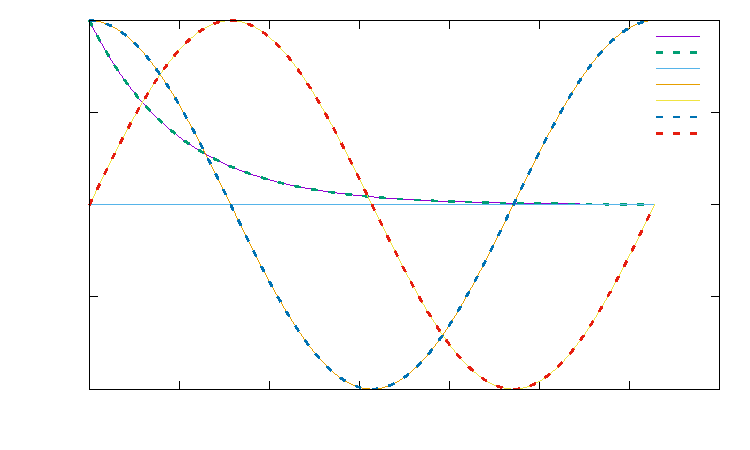
\includegraphics{plot_imag}}%
    \gplfronttext
  \end{picture}%
\endgroup

	\caption{Here the complex exponential gotten from the ODE-routine is plotted for two inputs: a purely imaginary one and a purely real one.
		The corresponding functions from math.h is included for comparison, showing that the routine works as intended for complex
		functions of complex variables. In the case of a purely real input to the complex exponential the resulting values are split into
		their real and imaginary parts for easy comparison.}
\label{fig:complex}
\end{figure}

\end{document}


